\makeatletter\frontmatter@init\makeatother

\title{Surface Treatment of Shallow, Proximitized InAs Quantum Wells}

\author{S. J. Pauka}
\author{J. Witt}
    \affiliation{ARC Centre of Excellence for Engineered Quantum Systems, School of Physics, The University of Sydney, NSW 2006, Australia.}
\author{C. N. Allen}
    \affiliation{Microsoft Quantum Sydney, The University of Sydney, Sydney, NSW 2006, Australia.}
\author{B. Harlech-Jones}
\author{A. Jouan}
    \affiliation{ARC Centre of Excellence for Engineered Quantum Systems, School of Physics, The University of Sydney, NSW 2006, Australia.}
\author{G. C. Gardner}
\author{S. Gronin}
\author{T. Wang}
\author{C. Thomas}
    \affiliation{Birck Nanotechnology Center, Purdue University, West Lafayette, IN 47907, USA.}
    \affiliation{Microsoft Quantum Purdue, Purdue University, West Lafayette, IN 47907, USA.}
\author{M. J. Manfra}
    \affiliation{Department of Physics and Astronomy, Purdue University, West Lafayette, IN 47907, USA.}
    \affiliation{Birck Nanotechnology Center, Purdue University, West Lafayette, IN 47907, USA.}
    \affiliation{Microsoft Quantum Purdue, Purdue University, West Lafayette, IN 47907, USA.}
    \affiliation{School of Materials Engineering and School of Electrical and Computer Engineering, Purdue University, West Lafayette, IN 47907, USA.}
\author{D. J. Reilly}
    \affiliation{ARC Centre of Excellence for Engineered Quantum Systems, School of Physics, The University of Sydney, NSW 2006, Australia.}
    \affiliation{Microsoft Quantum Sydney, The University of Sydney, Sydney, NSW 2006, Australia.}
\author{M. C. Cassidy}
    \affiliation{Microsoft Quantum Sydney, The University of Sydney, Sydney, NSW 2006, Australia.}

\makeatletter
\begingroup
\@author@finish
\frontmatter@author@produce@script
\endgroup
\makeatother

\begin{abstract}
    Proximitized 2-dimensional electron gasses (2DEGs) with strong spin-orbit interaction (SOI) such as InAs and InSb have been proposed as candidate materials for scalable topologically protected qubits. The need to form shallow quantum wells to create a hard-gapped $p$-wave superconducting state subjects them to fabrication induced damage, limiting the ultimate mobility in these samples. We study scattering mechanisms in InAs 2DEG quantum wells and demonstrate methods to repair the semiconductor/dielectric interface following processing to increase mobility. Passivation of charged impurity states with a ArH plasma results in a significant increase in the measured mobility and reduction in variance relative to untreated samples, up to \mob{45300} in a \SI{10}{\nano\meter} deep quantum well.
\end{abstract}

\subsection{\label{sec:surf_intro}Introduction}

Interest in proximitized 2-dimensional electron gasses (2DEGs) in InAs and InSb has intensified in recent years due to their potential applications in spintronics \cite{spintronics} and topological quantum computation \cite{PhysRevLett.105.077001,s41578-018-0003-1}. These materials can be proximitized by a superconductor deposited on their surface, which strongly couples to the quantum well. The induced superconductivity combined with strong SOI and a large Land\'e g-factor in these materials results in the formation of Majorana zero modes (MZMs) in nanowires \cite{Mourik1003,AlbrechtNature} and 2DEGs \cite{PhysRevLett.119.136803,PhysRevLett.119.176805}. MZMs are an emergent quasiparticle hypothesized to have non-abelian exchange statistics and may provide topological protection to quantum information \cite{RevModPhys.80.1083}, and are expected to emerge at the boundaries of topological superconductors \cite{RevModPhys.83.1057,Kitaev_2001,doi:10.1146/030212-184337}.

Early experimental realization of MZMs in both VLS nanowires and 2DEGs utilized superconductors deposited ex-situ; however, these systems demonstrated a large subgap density of states that obscured the signatures of the MZM \cite{PhysRevB.88.064506,PhysRevLett.110.186803}. In-situ deposition of a superconductor such as epitaxially grown aluminum directly after semiconductor growth resulted in a significant improvement in the quality of the superconducting gap \cite{nnano.2014.306,hard_gap_2deg}, and key results such as quantization of the zero bias peak \cite{nature26142}. However, this technique poses additional fabrication challenges, as the Al must be removed to define the topological region of the device. Wet etch solutions selective to Al are highly exothermic and result in damage to the surface of the semiconductor. This results in increased roughness and induced impurities, reducing the mobility of the 2DEG\footnote{From \mob{44000} \cite{shabani_transport} down to \mobr{1000}{2000} \cite{hard_gap_2deg,PhysRevLett.115.127001}} and compromising the fragile induced $p$-wave superconducting pairing \cite{PhysRevB.83.184520,PhysRevB.85.140513}. Because the length scale over which hard-gap superconductivity is maintained through a clean interface is set by the height and thickness of the barrier \cite{PhysRevLett.110.186803} burying the 2DEG deep in the heterostructure is not feasible \cite{PhysRevB.93.155402}, so new fabrication techniques that maintain or repair defects introduced at the surface must be developed.

Here we investigate the scattering mechanisms that reduce mobility in shallow InAlAs/InAs/InGaAs 2DEG heterostructures following wet etch of the proximitizing superconductor. By studying Hall mobility as a function of density, we show that surface scattering is the dominant mechanism for reduced mobility in shallow 2DEG samples. We demonstrate that the mobility can be increased and its variance reduced by exposing the sample to an in-situ ArH plasma prior to deposition of a protective ALD-grown \ce{Al2O3} coating, compared to samples exposed to a in-situ trimethylaluminum (TMA) pre-treatment prior to \ce{Al2O3} growth, or without any pre-treatment.


\begin{figure}
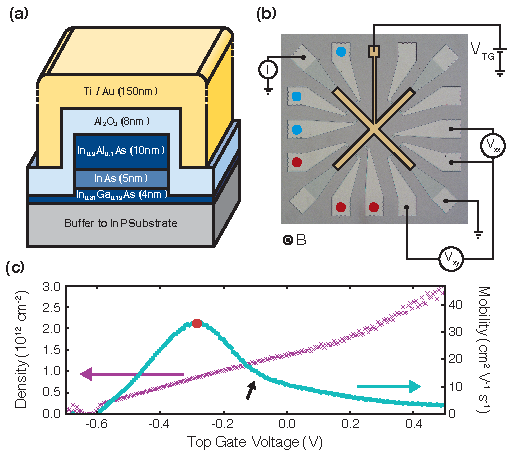
\includegraphics{Figure1}
\caption[InAs sample details and experimental setup]{\label{fig:surf_fig1} (a) Cross section of a shallow InAlAs/InAs/InGaAs quantum well after removal of epitaxially grown Aluminum. A protective layer of \ce{Al2O3} is grown, along with a \SI{150}{\nano\meter} Ti/Au surface gate which is used to tune the electron density. (b) False color micrograph and schematic of the experimental setup showing one combination of current and voltage contacts. Red and blue dots indicate alternative measurement points. (c) The density (violet) and mobility (cyan) of sample B are extracted from magnetoconductance measurements as the top gate is swept. The red mark indicates the location of peak mobility. The black arrow indicates the location of the second subband filling.}
\end{figure}

\subsection{\label{sec:surf_exp}Experiment}

The devices are fabricated from a InAlAs/InAs/InGaAs quantum well grown \SI{10}{\nano\meter} below the surface on a 2'' (100) InP substrate \cite{manfra_hmob}. An \SI{8}{\nano\meter} Al layer is grown epitaxially on the surface of the heterostructure directly following the semiconductor growth. On each sample, a Hall bar geometry is defined using a dilute phosphoric acid etch, and Al is selectively removed over the Hall bar with an Aluminum wet etch (Transene type-D). Contact to the 2DEG is made using sections of un-etched Al, which forms an ohmic contact. The surface is then treated using either TMA as a reducing agent to remove the native oxide \cite{ingaas_redux,iiiv_cleanup} or with a ArH plasma to terminate charged impurity states \cite{BELL1998125}, and without breaking vacuum, a \SI{10}{\nano\meter} \ce{Al2O3} oxide is grown via ALD at \SI{200}{\celsius}, using a TMA precursor and either \ce{H2O} or \ce{O3} as an oxidizing agent. Finally, a \SI{150}{\nano\meter} Ti/Au gate is evaporated on the surface of the Hall bar to allow the electron density of the samples to be varied. Further details of the fabrication are contained in the Supplementary Information. A cross-sectional schematic of the Hall bar is given in Fig.~\ref{fig:surf_fig1} (a). For each treatment/oxidizer pair, we fabricate two samples, one taken from within 1'' of the center of the wafer (denoted `near'), the other taken from the outer 1'' ring (denoted `far'), in order to account for variation in mobility as a function of distance from the center of the wafer \cite{watson_thesis}. A full list of tested sample parameters is given in Table~\ref{tab:surf_sampparam}. We note that despite the higher quality of ALD oxides grown at higher temperatures, at temperatures higher than \SI{250}{\celsius}, diffusion of In and As occurs, and above \SI{300}{\celsius} \ce{In} begins to precipitate out of the substrate due to the desorption of \ce{As} \cite{PhysRevB.48.2807}.

\begin{table}
\begin{centering}
\begin{tabular}{lll}
\toprule
Sample&
Treatment&
Precursor/Oxidizer\\
\midrule
A & No Treatment & TMA/\ce{H2O} \\
B & TMA Reduction & TMA/\ce{H2O} \\
C & TMA Reduction & TMA/\ce{O3} \\
D & \ce{H2} Passivation & TMA/\ce{H2O} \\
E & \ce{H2} Passivation & TMA/\ce{O3} \\
\bottomrule
\end{tabular}
\caption[InAs sample treatments and growth parameters]{\label{tab:surf_sampparam}%
A full listing of sample growth parameters that were tested. Two surface treatments (TMA Reduction and \ce{H2} Passivation) and two oxidizers (\ce{H2O} and \ce{O3}) are tested to find their effect on sample mobility. Each treatment and oxidizer pair are measured on two chips, one taken from the center of the growth wafer, the other from near the edge, in order to account for the effect of distance from the center of the wafer on mobility.}
\end{centering}
\end{table}

Measurements were carried out in a dilution refrigerator with a base temperature of \SI{7}{\milli\kelvin}. Magnetotransport measurements were performed to extract electron densities and mobilities using conventional AC lock-in techniques, with a \SI{10}{\nano\ampere} constant current. A representative Hall bar is shown in Fig.~\ref{fig:surf_fig1} (b), with longitudinal ($R_{xx}$) and transverse ($R_{xy}$) resistance measured simultaneously. Three measurement points are defined around the edge of the Hall bar, indicated with blue, red and black dots, allowing multiple independent measurements of mobility and density to be made on each sample, from which statistics on each treatment are gathered. Hall bars were oriented at $\ang{45}$ to the $(011)$ and $(01\overline{1})$ plane to remove effects of any anisotropy along different crystallographic axes \cite{PhysRevB.67.045309,PhysRevB.77.235307}. For each sample, density and mobility are extracted as the top gate is swept. A representative measurement is shown for sample B, taken from near the center of the growth wafer, in Fig.~\ref{fig:surf_fig1} (c). Mobility is extracted at \SI{0.05}{\tesla}, which is a sufficiently large offset to ensure we are no longer on the weak-antilocalization peak. A peak value for mobility is extracted of \mob{33400} at a density of \den{8.73e11}, corresponding to a gate voltage of $V_{TG} = \SI{-0.27}{\volt}$, and indicated by the red point in Fig.~\ref{fig:surf_fig1} (c). We can attribute different dominant scattering mechanisms to various ranges of the density \cite{Matsumoto_1974,PhysRevB.32.8126,PhysRevB.16.4446}. As the density increases from zero, scattering is predominantly caused by scattering off background impurities distributed through the heterostructure \cite{scattering}. Increased screening of impurities as the density is increased leads to an increase in mobility. As the gate voltage and density is further increased, the mobility is seen to peak, before reducing with increasing density. Increasing top gate voltage causes the the distribution of electrons in the quantum well to shift towards the surface \cite{doi:10.1063/1.119829,PhysRevB.93.235312}, and surface scattering becomes dominant over the increased impurity screening with higher density, leading to a decrease in mobility as the density is further increased.


\begin{figure}
    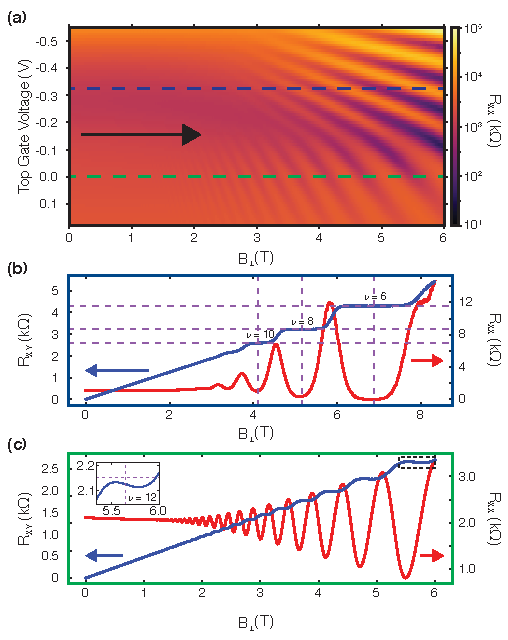
\includegraphics{Figure2}
    \caption[Magnetoresistance measurements and Landau fan for sample B]{\label{fig:surf_fig2}(a) The Landau fan for sample B. The black arrow marks the onset of second subband population, indicated by a change in slope of the Landau levels as a function of magnetic field and top gate voltage. The location of peak mobility is indicated by the blue dashed line. (b) Magnetoresistance taken at the point of highest mobility on sample B. Well resolved hall plateaus are observed, starting from $\nu = 10$ (see main text for details). (c) Magnetoresistance measurements of sample B to high field, taken at $V_{TG} = \SI{0}{\volt}$. Hall plateaus show an oscillation characteristic of parallel conduction paths. }
\end{figure}

 Figure~\ref{fig:surf_fig2} (a), shows a Landau fan for sample B measured in a second cooldown, plotting $R_{xx}$ as $V_{TG}$ and $B$ are swept.  The onset of second subband population is marked by the arrow and occurs at $V_{TG} = \SI{-0.16}{\volt}$, denoted by the change in the slope of the location of Landau levels as a function of gate voltage and magnetic field \cite{PhysRevB.74.195313,STORMER1982707}, and indicated by the black arrow on Fig.~\ref{fig:surf_fig1} (c). This is caused by a reduction in the rate of filling of the first subband $N_{S1}$ relative to the total density $N_T = N_{S1} + N_{S2}$.

The sample shows significantly different magnetotransport behavior when the first and second subbands are occupied. When the top gate is tuned to the value that maximizes mobility at zero magnetic field, $V_{TG} = \SI{-0.32}{\volt}$ (Fig.~\ref{fig:surf_fig2}~(b)), well resolved Hall plateaus are observed from $\nu = 10$ onwards, with the Hall resistivity quantized to within $0.11\%$ of the theoretical value at $\nu = 6$, and a vanishing longitudinal resistance of $R_{xx} = \SI[per-mode=symbol]{2.4}{\ohm\per\sq}$. No Shubnikov-de Haas oscillations are observed. In contrast, when the second subband is occupied at $V_{TG} = 0$ (Fig.~\ref{fig:surf_fig2} (c)), clear Shubnikov-de Haas oscillations are visible to \SI{6}{\tesla}, despite the much lower mobility of the sample at this point. This effect has been observed in previous measurements of low-mobility GaAs and is caused by the increased screening of the impurity potential by the electrons of the second subband \cite{PhysRevB.38.7866}. An oscillation of Hall resistivity is observed on plateaus and is attributed to parallel transport in the second subband (inset Fig.~\ref{fig:surf_fig2} (c)). We note that the filling of the second subband at $V_{TG} = \SI{0}{\volt}$ is a potential complicating factor in the search for Majoranas in InAs 2DEG \cite{s41578-018-0003-1}.

\subsection{\label{sec:surf_treat}Surface Treatments and Oxide Growth}

\begin{figure}
    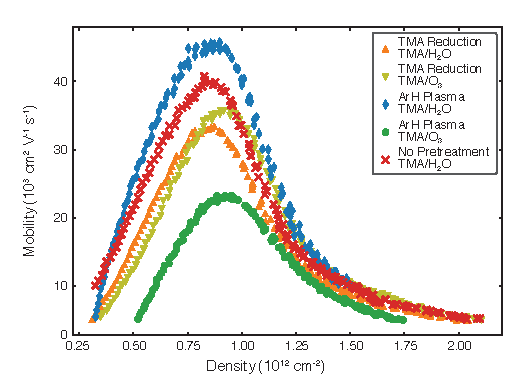
\includegraphics[width=0.6\linewidth]{Figure3}
    \caption[Representative mobility vs. density traces for each treatment]{\label{fig:surf_fig3} Representative mobility vs. density traces for each treatment, taken from samples near the center of the wafer. Samples oxidized with \ce{O3} show a shifted peak mobility relative to those oxidized with \ce{H2O}. A peak mobility of \mob{45300} is extracted for a sample treated with a Hydrogen plasma.}
\end{figure}

The native oxide layer in both GaAs and InAs is known to contain a large number of charged defects \cite{doi:10.1063/1.5054292,PhysRevB.49.11159}, caused by unpaired As atoms within the oxide formed by an excess of As during the oxidation of In and Ga \cite{doi:10.1063/1.3369540,Affentauschegg_2001}. The presence of these scattering sites at the surface of the wafer limits the mobility of samples above a certain density. Reducing the density of surface scattering sites through chemical treatment prior to dielectric deposition provides a clear pathway to increasing the sample mobility. There is an extensive history of the repair of the surface of III-V materials by either reduction with TMA, or utilizing atomic hydrogen cleaning.

The first approach examined is the removal of the native oxide through reduction by TMA, allowing the growth of abrupt semiconductor/dielectric interfaces with a reduced defect density \cite{doi:10.1063/1.3148723,Tallarida_2012,CLEVELAND2013167}.
TMA is known to remove the surface oxides of InAs via the following reaction \cite{iiiv_cleanup}:
\begin{align}
    \ce{2Al(CH3)3 + In2O3 &-> 2In(CH3)3 + Al2O3} \\
    \ce{2Al(CH3)3 + As2O3 &-> 2As(CH3)3 + Al2O3}
\end{align}

For TMA treated samples, a \SI{1}{\second} pulse of TMA is applied to the surface in the ALD chamber, followed by a \SI{30}{\second} purge with \ce{N2} gas, at a \SI{200}{\celsius} process temperature. This pulse cycle is repeated 18 times to maximize the reaction time, prior to the growth of the dielectric.

The second approach that we examine is the removal of surface oxides and the passivation of charged impurities at the surface via the application of an ArH plasma to the chip \cite{CLEVELAND2013167,BELL1998125,doi:10.1116/1.586538}. For this process, a remotely generated ArH plasma is applied to the surface of the samples for a total of \SI{120}{\second} before the growth of the dielectric layer. Atomic hydrogen is known to bond to As atoms and saturate the dangling bonds, passivating the surface. A hydrogen plasma is also known to selectively remove the surface oxide via dry etching, again leading to an abrupt semiconductor-dielectric interface \cite{doi:10.1063/1.92194,doi:10.1063/1.100961}.

\begin{figure}
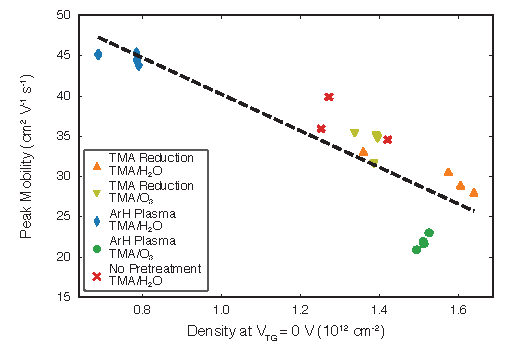
\includegraphics[width=0.6\linewidth]{Figure4}
\caption[Peak mobilities for different treatments and oxidizers]{\label{fig:surf_fig4} Peak mobility achieved for different treatment and oxidizers. Measurements are made across different two samples, taken from near the center of the growth wafer (green) and from near the edge of the growth wafer (red), and at multiple locations on each Hall bar. Each point represents the peak mobility extracted from a sweep of gate voltage, as shown in red in Fig.~\ref{fig:surf_fig1} (c), which were collected over multiple cooldowns, and at multiple measurement points.}
\end{figure}

For each sample, $V_{TG}$ is swept, and mobility and density are extracted. In Fig.~\ref{fig:surf_fig3} we plot mobility as a function of density for each treatment, with samples taken from near the center of the wafer. The use of ArH plasma in combination with oxide growth using TMA and \ce{H2O} as an oxidizer was found to increase the measured mobility relative to an untreated sample, showing the highest peak mobility for both near and far samples. In contrast, oversaturation with TMA causes a decrease in mobility compared to a single TMA exposure before \ce{Al2O3} growth. We hypothesize this is because the interface oxide that is grown in the place of the native oxide is not significantly cleaner relative to the removed native oxide.  Finally, we note that the use of \ce{O3} as a precursor does not seem to be effective for the creation of a clean dielectric interface -- both ozone samples show a decreased quality relative to no treatment, however the peak mobilty shifts to a higher density. Previous studies have indeed found that the \ce{AlO_x} grown is oxygen-rich relative to the optimal stoichiometry for aluminum oxide and leads to a lower quality oxide \cite{ingaas_redux,10.1021/cm0608903}.  A summary of results is shown in Fig.~\ref{fig:surf_fig4}. Measurements are taken on both samples near the center of the growth wafer (near) and samples taken far from the center of the growth wafer (far), across multiple measurement points and multiple cooldowns. As expected, there exists a significant gap in the mobility of samples taken from different parts of the growth wafer, however, there remains a definite trend amongst similarly treated samples.

\subsection{\label{sec:surf_scat}Scattering Mechanisms}

\begin{figure}
    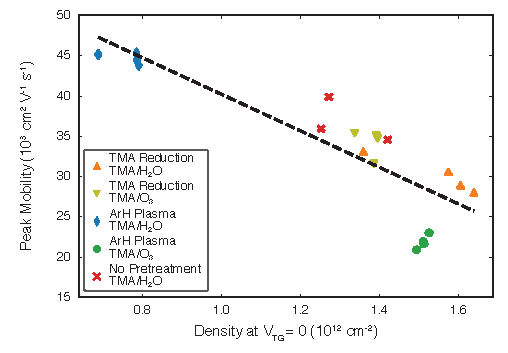
\includegraphics[width=0.6\linewidth]{Figure5}
    \caption[Density at zero gate voltage vs. peak mobility]{\label{fig:surf_fig5}Scatter plot of density at zero gate voltage against the peak mobility, for samples taken near the center of the growth wafer. Samples with the lowest density at zero gate voltage have the highest measured peak mobility. The dashed black line is a linear fit, and is a guide to the eye.}
\end{figure}

Finally, we turn to a detailed examination of scattering mechanisms across different density ranges and surface treatments. First, we examine the role of interface scattering at charged surface states in limiting the mobility of shallow InAs quantum wells. To extract the densities of charged surface states, we note that the samples studied are all undoped. Unlike semiconductors such as GaAs where the Fermi level is pinned in the band gap, the location of the Fermi level in InAs has been shown to depend sensitively on surface states, and an electron density in the quantum well at zero gate voltage is induced by charged impurities at the surface \cite{PhysRevLett.66.2243,Affentauschegg_2001}. As the density of charged impurities is decreased, the electron density in the quantum well at zero gate voltage is decreased towards zero. Fig.~\ref{fig:surf_fig5} shows the density at zero gate voltage against the peak mobility. We find there is an inverse relationship, and observe that the samples with the highest mobility have the lowest intrinsic electron density. We can conclude that scattering off charged surface impurities is a limiting factor in mobility in the current generation of shallow quantum wells, and that an atomic hydrogen plasma is an effective method for terminating these charged impurities. In contrast, we find that samples treated with TMA see either no significant change in the density of charged surface states or see an increase relative to no pre-treatment. Although TMA treatments should be effective in cleaning the surface oxide, we note that previous studies have been carried out at much higher temperatures, and in this case the repeated TMA pulsing may leave an excess of TMA bonded to the surface and hamper clean ALD growth.

To explain the observed damage caused by the use of Ozone as an oxidizer, we examine the relationship between density and mobility when peak mobility is achieved (See supplementary for additional data). A shift is visible between those samples that use \ce{H2O} and those that use \ce{O3} as an oxidizer, with \ce{O3} samples shifted towards higher densities. We propose that this is caused by the increased incorporation of oxygen in the oxide \cite{10.1021/cm0608903}, which appear as remote charged impurity scatterers \cite{scattering} distributed throughout the dielectric. Such scattering sites are screened by electrons in the 2DEG as the electron density is increased, which, due to the higher concentration of remote charged impurities in the sample, requires a larger electron density to screen.

\subsection{Conclusion}
In summary, we study the scattering mechanisms in shallow InAs 2DEGs and demonstrate that the application of an ArH plasma prior to dielectric growth is effective in reducing the density of charged surface states at the \ce{InAs}/\ce{Al2O3} interface. For a quantum well \SI{10}{\nano\meter} from the surface, this results in an increase in peak mobility to $\sim \mob{45000}$, and a reduction in variance compared to untreated samples.

\subsubsection{Acknowledgments}
This research was supported by the Microsoft Corporation and the Australian Research Council Centre of Excellence for Engineered Quantum Systems (EQUS, CE170100009). The authors acknowledge the facilities as well as the scientific and technical assistance of the Research \& Prototype Foundry Core Research Facility at the University of Sydney, part of the Australian National Fabrication Facility
